\section{Tree-like modes of hashing}
Consider an \(n\)-bit CHF \(H\), and suppose that a prover claims to know some message \(m\): 
the digest \(d = \call{H}{m}\) can be considered as a \emph{short binding commitment} for \(m\): 
By asking the prover to share the digest, whose size \(\abs{d} = n\) is typically considered to be 
\(\BigO{1}\) (or \(\BigO{\call{\log}{\abs{m}}}\) in some cases), a verifier is convinced that the 
prover does know \(m\) with probability \(\approx 1 - {1}/{2^n}\).
A modern standard CHF like SHA-256~\cite{Dang2015} produces digests of length at least \(256\) bits,
making the \(1 - {1}/{2^n}\) bound really hard to bruteforce through.
Note that the verifier needs not to know \(m\) in advance: the commitment \(d\) is (temporarily) 
appended to a public \emph{blockchain} and, at any point in the future, when the verifier becomes 
aware of some \(m'\) provided by the prover, if \(\call{H}{m'} = d\), the commitment can be 
approved or rejected.

Now, suppose that the prover wants to commit to a list of \(k\) messages: the simplest solution 
would be to publish the hash of every message, which would require to append \(\BigO{k}\) 
elements on the blockchain.
Another way would be for the prover to share \(\call{H}{\Tuple{m_1, \dots, m_k}}\): the 
communication cost would only be \(\BigO{1}\) but, in general, not all the messages belong to the 
same prover, so this method would not work, and we need a better solution.

\subsection{Merkle tree}
\begin{definition}[Binary Merkle tree~\cite{Merkle1988}]
	A \emph{binary Merkle tree (MT)} of height \(h \in \mathbb{N}\) over a \(2n\)-to-\(n\) compression 
	function \(C\), is the complete binary tree of height \(h\) such that, given a sequence of input 
	messages \(\Tuple{m_1, \dots, m_{2^{h-1}}}\) over \(\Set{0, 1}^{2n}\), produces an
	output digest \(d \in \Set{0, 1}^{n}\) in the following way:
	\begin{enumerate}
		\item The leaf nodes \(\nu_1, \dots, \nu_{2^{h-1}}\) contain 
					\(\call{C}{m_1}, \dots, \call{C}{m_{2^{h-1}}}\).
		\item Every other node \(\nu \) contains \(\call{C}{\nu_l, \nu_r}\), where \(\nu_l\) is
		      the left child of \(\nu \) and \(\nu_r\) is the right child of \(\nu \).
		\item The output digest \(d\) is the content of the root node. 
	\end{enumerate}
\end{definition}

By using Merkle trees, the prover only needs to send to the verifier, as a commitment for
some message \(m_i\) among \(n = 2^h\) messages, the contents of the co-path from the leaf 
containing \(m_i\) to the root, in addition plus the hash of \(m_i\): this requires
just \(\BigO{\call{\log}{n}}\) cost to validate the commitment.
Merkle trees bottom-up construction is very easy to parallelize, and they can be used in the 
multiple-provers scenario: each prover only needs to commit to the path from its own leaf to the 
root of the tree.
It is immediate to generalize the notion of binary Merkle tree to arbitrary arity.
\begin{proposition}[Security of Merkle tree mode of hash~\cite{Merkle1988}]
	Given a one-way \(tn\)-to-\(n\) compression function \(C\), the \(t\)-ary Merkle tree over 
	\(C\) is a cryptographic hash function.
\end{proposition}

\begin{example}\label{ex:merkle_tree}
	Consider the sequence of messages \(S = \Tuple{3, 4, 7, 7}\) and the compression function 
	\(\call{C}{x, y}: \Tuple{x, y} \mapsto xy \bmod 13\) (for ease of exposition, we work over 
	integers instead of bit strings, but the two can be readily converted into one another).
	\Cref{fig:merkle_tree} shows the contents of the associated Merkle Tree.
\end{example}
\begin{figure}
	\centering
		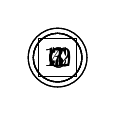
\begin{tikzpicture}[sibling distance=32pt, level distance=32pt]
			\tikzset{edge from parent/.style={draw, <-, edge from parent path=
					{(\tikzparentnode) -- (\tikzchildnode)}}}
			\Tree 
			[
				.\node[draw,circle]{3};
				[
					.\node[draw,rectangle]{C};
					[
						.\node[draw,circle]{12};
						[
							.\node[draw,rectangle]{C};
							[
								.\node[draw,circle]{3};
%								[
%									.\node[draw,rectangle]{C};
%									[
%										.\node[]{42};
%									]
%								]
							]
							[
								.\node[draw,circle]{4};
%								[
%									.\node[draw,rectangle]{C};
%									[
%										.\node[]{69};
%									]
%								]
							]
						]
					] 
					[
						.\node[draw,circle]{10};
						[
							.\node[draw,rectangle]{C};
							[
								.\node[draw,circle]{7};
%								[
%									.\node[draw,rectangle]{C};
%									[
%										.\node[]{07};
%									]
%								]
							]
							[
								.\node[draw,circle]{7};
%								[
%									.\node[draw,rectangle]{C};
%									[
%										.\node[]{33};
%									]
%								]
							]
						]
					]
				]
			]
			\end{tikzpicture}
	\caption{Merkle tree of \Cref{ex:merkle_tree}.}\label{fig:merkle_tree}
\end{figure}

\subsection{Augmented Binary Tree}
The Merkle tree is the de-facto standard for blockchain applications, and basically for any 
scenario for which a `linear' hash function cannot be used.
In~\cite{Stam2008}, it was given a lower bound on the amount of queries necessary to obtain a 
collision for a \(\Parens*{m+s}\)-to-\(s\)-bit CHF \(H\) (the \(m\) is variable) built from a 
\(\Parens*{n+c}\)-to-\(n\)-bit OWCF \(C\): if \(H\) makes \(r\) queries to \(C\), it is possible 
to find a collision by making \(2^{\frac{nr + cr - m}{r + 1}}\) queries to \(H\).
By combining this result with the \(2^{s/2}\) upper bound of the birthday paradox, one can 
immediately obtain a tight bound \(m = \frac{2nr + 2cr -sr - s}{2}\) for the variable length \(m\) 
of the message.

\begin{definition}[Compactness~\cite{AndreevaBR2021}]
	The \emph{compactness} of an \(\Parens*{m+s}\)-to-\(s\)-bit hash function making \(r\) queries to 
	an underlying \(\Parens*{n+c}\)-to-\(n\)-bit one-way compression function is the value
	\(\alpha = \frac{2m}{2nr + 2cr -sr - s}\).
\end{definition}

\begin{example}\label{ex:mtree_compactness}
	Consider a \(2n\)-to-\(n\) bit OWCF and a Merkle Tree of height \(h\): the computation 
	of the tree is a \(\Parens*{2^{h-1}n}\)-to-\(n\)-bit hash function, and makes exactly 
	\(r = 2^{h-1} - 1\) queries to \(C\).
	We have \(s = c = n\) and \(m = 2^{h-1}n - n = nr\), therefore the compactness of the Merkle 
	Tree construction is:
	\[
		\alpha = \frac{2m}{2nr + 2cr -sr - s} = 
		\frac{2nr}{2nr + 2nr - nr - n} =
		\frac{2r}{3r - 1}
	\]
	Which tends to \(2/3\) when \(r\) tends to infinity.
\end{example}

\begin{definition}[Augmented Binary tRee~\cite{AndreevaBR2021}]
	An \emph{Augmented Binary tRee (ABR)} of height \(h \in \mathbb{N}\) over a 
	\(2n\)-to\(n\) compression function \(C\) is a complete binary tree of height \(h\) 
	augmented with \emph{middle} nodes such that, given a sequence of input messages
	\(S = \Tuple{m_1, \dots, m_{2^{h-1} + 2^{h-2}-1} \mid \forall i\colon m_i \in \Set{0, 1}^{*}}\), 
	it produces an output digest \(d \in \Set{0, 1}^n\) in the following way:
	\begin{enumerate}
		\item The leaf nodes \(\nu_{1}, \dots, \nu_{2^{h-1}}\) contain \(\call{C}{m_1}, \dots,
		      \call{C}{m_{2^{h-1}}}\).
		\item There are no middle nodes in the leaf layer.
		\item The middle nodes \(\nu_{2^{h-1}+1}, \dots, \nu_{\abs{S}}\) contain
		      \(\call{C}{m_{2^{h-1}+1}}, \dots, \call{C}{m_{\abs{S}}}\).
		\item Every other node \(\nu \) contains \(\call{C}{\nu_l \oplus \nu_m, \nu_r \oplus
		      \nu_m} \oplus \nu_r \), where \(\nu_l\) is the left child of \(\nu \), \(\nu_r\)
		      is the right child of \(\nu \), and \(\nu_m\) is the middle child of \(\nu \), or \(0\)
		      if \(\nu \) doesen't have a middle child.
	\end{enumerate}
\end{definition}

\begin{proposition}[Security of ABR mode of hash~\cite{AndreevaBR2021}]
	Given a one-way \(2n\)-to-\(n\) compression function \(C\), the ABR over \(C\) is a cryptographic 
	hash function.
\end{proposition}

An ABR of height \(h\) can process 50\% more messages than a Merkle Tree of the same height, 
while performing the same number of queries to the underlying compression function, with the 
additional cost introduced by the intermediate \(\oplus \) operations being negligible in most 
scenarios.

\begin{example}
	Consider a \(2n\)-to-\(n\) bit OWCF and an ABR of height \(h\): the computation 
	of the tree is a \(\Parens*{2^{h-1} + 2^{h-2}-1}n\)-to-\(n\)-bit hash function, 
	and makes exactly \(r = 2^{h-1} - 1\) queries to \(C\).
	Like in \Cref{ex:mtree_compactness}, we have \(s = c = n\), but this time 
	\(m = \Parens*{2^{h-1} + 2^{h-2}-1}n - n = nr + {nr}/2 - n\), so the compactness of the ABR 
	construction is:
	\[
		\alpha = \frac{2m}{2nr + 2cr - sr - s} = 
		\frac{2nr + nr - 2n}{2nr + 2nr - nr - n} =
		\frac{3r - 2}{3r - 1}
	\]
	Which approaches \(1\) as \(r\) approaches infinity, meaning that the ABR construction achieves
	optimal compactness.
\end{example}

It is worth of notice that, while the ABR hash mode achieves collision resistance, it does not 
achieve \emph{indifferentiability} (a weaker notion of indistinguishability between Turing 
machines~\cite{MaurerRH2003}), hence a modified construction, called ABR+, was also proposed, at 
the cost of reduced compactness (however still higher than a Merkle tree).
